\chapter{Scale, Control, and the Architecture of Real-Estate Wealth}

This lecture begins by refusing to explain itself. It first shows us scale in raw form: a Bugatti, a skyline, and a casually stated year of almost five billion dollars. Only after that opening shock does it begin to unfold its argument. The movement is deliberate. We pass from visible wealth to the city that makes such wealth intelligible, from the city to a building, from the building to real estate as an asset class, from the asset class to vertical integration, and from there to the deeper themes of quality, people, consistency, legacy, and faith. The mathematics here is not the mathematics of a chalkboard; it is the mathematics of scale, control, and compounding.

\section{Scale Before Explanation}

The first move of the lecture is to establish abnormal magnitude before giving us any theory at all. We are shown a Bugatti, and the implied question is immediate: what sort of commercial machine must exist behind so visible a piece of wealth? The interview then sharpens the point with a coarse numerical marker:
\begin{equation}
Y_{\max} \approx \$5 \times 10^{9}.
\end{equation}
Here \(Y_{\max}\) denotes the speaker's self-reported largest amount of money made in a single year.

\begin{remark}
The transcript gives this number as an approximate range offered from memory. We therefore preserve the scale of the claim while leaving unresolved whether it refers to profit, income, realized gains, or some broader business measure.
\end{remark}

The important thing is not accounting precision. The important thing is narrative order. First the lecture shocks us. Then it tells us where that shock belongs. ``This is Dubai'' is not merely geographical background; it is the lecture's first explanatory sentence. Dubai is presented as a place where billion-dollar deals are made over coffee, where the skyline is itself a record of concentrated entrepreneurial ambition, and where wealth operates on a different order of magnitude.

That widening of the frame is crucial. If the number were left alone, it would remain a curiosity. By embedding it in the city, the lecture turns a private claim into an environmental fact. The host's sixteen-hour trip is then used to give that fact weight. We are supposed to feel that this is not casual tourism; it is a journey into a field where scale itself is the first lesson.

\section{The Building as Evidence}

The lecture then does something equally important: it refuses to let scale float free of proof. The host does not simply stay in the register of city mythology. He travels to the Bugatti Residences and repeatedly names the place. We are told that this is the first Bugatti Residence in the world, that the Burj Khalifa stands nearby as an anchor of urban ambition, and that the speaker is not a commentator on luxury construction but one of its makers.

So the order is now very clear. First the lecture gives us scale. Then it gives us setting. Then it gives us a product inside the setting. Before theory, there is location. Before principle, there is evidence.

\subsection{Question \& Answer}

\paragraph{Question.} How does someone become credible enough to build with one of the biggest luxury brands in the world?

\paragraph{Answer.} Mohamed's first answer is not financial and not technical. It is temperamental. Passion goes into it, he says. One has to be obsessed. One wakes up every day obsessed with the goal and willing to grind. In the lecture's order, this matters a great deal. We do not begin with negotiation strategy or partnership structure. We begin with intensity.

That answer is then reinforced by a small biographical turn. He recalls having Bugatti posters in his room as a child and says he never imagined he would achieve something like this. The point of that memory is not sentimentality. It is to show that the branded tower is the endpoint of a long line of desire, discipline, and persistence.

But the lecture does not remain inside biography. Once obsession has been named as the inner driver, the host pivots outward again and asks about place: why stay in the UAE, and why is this city such a fertile site for business?

\section{From Entrepreneurial Atmosphere to Asset Choice}

Mohamed's answer about Dubai is institutional. The city, in his view, possesses entrepreneurial flair, and the leadership has helped create an atmosphere that supports entrepreneurs in building billion-dollar businesses. That is the positive side of the environment. The lecture immediately balances it with the negative side. The host asks about no's, failures, and downsides, and Mohamed answers without hesitation: plenty.

That insertion of rejection is not incidental. It performs a necessary correction. If Dubai is presented only as a city of visible success, the lesson becomes too theatrical. By placing failure before the real-estate discussion, the lecture teaches that success is not the absence of resistance. It is the maturity to expect resistance and to navigate toward the answer one wants anyway.

Only after that moral and psychological preparation does the lecture ask its first major economic question: why real estate rather than some other vehicle?

\subsection{Question \& Answer}

\paragraph{Question.} Why do wealthy people keep ending up in real estate?

\paragraph{Answer.} Mohamed gives the answer in two layers. First comes the broad practical claim:
\begin{equation}
W_{\text{large}} \Longrightarrow A_{\text{RE}},
\end{equation}
where \(W_{\text{large}}\) denotes large accumulated wealth and \(A_{\text{RE}}\) a substantial real-estate allocation.

We should not read this as a theorem of finance. It is the lecture's strong practical rule: people who make a great deal of money tend to end up buying real estate. The second layer is the mechanism:
\begin{equation}
\text{tangibility} + \text{lower volatility} + \text{risk-manageability}
\Longrightarrow
\text{real-estate preference}.
\end{equation}

The vocabulary here is simple and revealing. Real estate is solid. One can touch it, feel it, see it, smell it. It is treated as less volatile than other assets and therefore as safer, or at least more legible, when the problem becomes not merely how to make money but where to hold it, store it, and compound it.

\paragraph{Anecdote.} The host asks why real estate was the chosen vehicle, as though many other vehicles had been available.

\paragraph{Claim.} Real estate is the asset class into which large wealth eventually settles.

\paragraph{Mechanism.} Its physicality and perceived stability make it an attractive resting place for capital.

This is the first true spine of the lecture. We have passed from spectacle into asset logic.

\section{Diversification Means Going Deeper}

Once real estate has been identified as the preferred asset, the lecture asks the next question almost automatically: how does one expand inside such a field? Here the interview produces one of its strongest ideas. Mohamed says that he did diversify, but learned a hard lesson: diversification does not always mean moving into another sector. One can diversify inside one sector by taking deeper control of its chain.

\begin{definition}
In the language of this lecture, vertical integration means that the developer does not remain only at the level of concept, branding, land, and sales. He progressively takes ownership of the production chain that makes the final product possible.
\end{definition}

The lecture's redefinition of diversification can therefore be compressed into
\begin{equation}
\text{diversification} \neq \text{necessarily new sector},
\qquad
\text{diversification} = \text{deeper control along one chain}.
\end{equation}

Mohamed then gives the redefinition operational content. They became completely vertically integrated as a developer. They built a construction company. They maintained their own workforce. They established factories, and the transcript is explicit enough to preserve at least the scale of that layer:
\begin{equation}
N_{\text{factories}} = 7.
\end{equation}
Joinery, aluminum, and steel are named in the interview; beyond that we should not invent a more elaborate taxonomy than the transcript supports.

The central middle claim of the lecture may then be written as
\begin{equation}
V_{\text{int}}
=
\{\text{construction},\ \text{in-house workforce},\ \text{factories}\}
\Longrightarrow
(\text{speed},\ \text{quality},\ \text{cost control}),
\end{equation}
where \(V_{\text{int}}\) denotes the depth of vertical integration.

\begin{figure}[h]
\centering
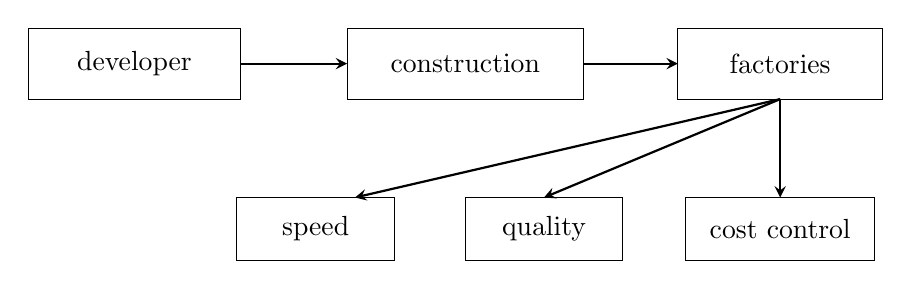
\begin{tikzpicture}[x=1cm,y=1cm,>=stealth]
\node[draw, rectangle, minimum width=2.7cm, minimum height=0.9cm] (dev) at (0,0) {developer};
\node[draw, rectangle, minimum width=3.0cm, minimum height=0.9cm] (con) at (4.2,0) {construction};
\node[draw, rectangle, minimum width=2.6cm, minimum height=0.9cm] (fac) at (8.2,0) {factories};

\draw[->, thick] (1.35,0) -- (2.7,0);
\draw[->, thick] (5.7,0) -- (6.9,0);

\node[draw, rectangle, minimum width=2.0cm, minimum height=0.8cm] (spd) at (2.3,-2.1) {speed};
\node[draw, rectangle, minimum width=2.0cm, minimum height=0.8cm] (qua) at (5.2,-2.1) {quality};
\node[draw, rectangle, minimum width=2.4cm, minimum height=0.8cm] (cost) at (8.2,-2.1) {cost control};

\draw[->, thick] (8.2,-0.45) -- (2.8,-1.7);
\draw[->, thick] (8.2,-0.45) -- (5.2,-1.7);
\draw[->, thick] (8.2,-0.45) -- (8.2,-1.7);
\end{tikzpicture}
\end{figure}

This figure is not a reconstruction of a visible on-screen diagram. It is an editorial condensation of what the speaker actually says. The business becomes faster, better, and more cost-aware to the extent that more of its decisive stages are brought inside the house.

\subsection{Question \& Answer}

\paragraph{Question.} What does diversification mean if leaving the sector is not the right move?

\paragraph{Answer.} It means reducing exposure to the chain by thickening one's ownership of the chain. One does not flee complexity. One internalizes the most consequential parts of it.

This is why the lecture's language about a single monstrosity of a business is so apt. The company does not scatter itself across unrelated opportunities. It enlarges its command of one immense commercial organism.

\section{Iteration Rather Than Perfect Planning}

The host then asks the right follow-up question. If the integrated machine contains construction, workforce, and factories, how does one actually arrive there? Surely nobody begins with the whole structure already in hand.

Mohamed's answer is one of the most coherent in the interview. One never has the full picture from day one, he says. One starts and navigates through. The bee begins its day without a full plan. It goes out and harvests. The bird does not begin with a completed map of the sky. And if one is thrown into the ocean in a storm, one either drowns or swims.

These are not decorative metaphors. They are the lecture's account of entrepreneurial method.

\subsection{Question \& Answer}

\paragraph{Question.} How do we scale when we do not yet know the full map from day one?

\paragraph{Answer.} We scale iteratively. A cautious bookkeeping model of the process is
\begin{align}
V_0 &= \{\text{development}\},\\
V_1 &= V_0 \cup \{\text{construction}\},\\
V_2 &= V_1 \cup \{\text{factories}\},\\
V_{n+1} &= V_n \cup \{\text{next bottleneck to internalize}\}.
\end{align}
If we let \(\mathcal{C}\) denote the full chain required to deliver the product, then a natural measure of outside dependence is
\begin{equation}
E_n = \lvert \mathcal{C} \setminus V_n \rvert.
\end{equation}
As \(V_n\) grows, \(E_n\) falls. In plain language: the more decisive functions the firm can perform itself, the fewer critical interfaces remain exposed to outside delay or outside quality variation.

The lecture gives the same idea in a more vivid and less symbolic form:
\begin{equation}
\text{start} \to \text{navigate} \to \text{fail} \to \text{fix} \to \text{figure out a way}.
\end{equation}

\paragraph{Worked example.} Suppose the business begins only at the development layer. Then all serious building execution lies outside the firm. Once construction is brought in-house, one major class of coordination delay is reduced. Once factories are added, additional material bottlenecks and fabrication dependencies are reduced as well. The chain is not invented whole; it is discovered through friction.

That is why the lecture places this answer exactly here. After hearing about seven factories and complete integration, we might imagine a perfectly designed empire from the beginning. Mohamed insists on the opposite picture. The empire is navigated into.

\section{Product, Design, and the Proof of Quality}

At this point the lecture returns to the building itself, but now the building appears not merely as prestige but as evidence. The site walk turns the middle theory into numbers:
\begin{align}
L_{\text{cladding}} &= 13\,\mathrm{km},\\
N_{\text{stories}} &= 46, \qquad N_{\text{units}} = 180,\\
A_{\text{penthouse}} &\approx 50{,}000\,\mathrm{ft}^2, \qquad N_{\text{car elevators}} = 2,\\
P_{\text{penthouse}} &= 750 \times 10^{6}\,\mathrm{AED}
\approx 2 \times 10^{8}\,\mathrm{USD}.
\end{align}

These figures do not constitute engineering blueprints, but they do serve a very definite function in the lecture. They show what vertical integration and design ambition look like when they harden into product. The triplex Crown Penthouse, the car elevators, the Riviera-inspired beach, the bespoke units: these are not random luxuries. They are the form taken by a business that wants its product to carry its own argument.

That is why the lecture next turns to speed and quality. Mohamed is described as one of the fastest developers in the region. When the host asks for the secret of that speed, the answer takes us back to the same center: vertical integration. Speed is not treated as a personality trait. It is treated as a structural consequence of control.

The interview then asks what has changed across the building record. Mohamed says the biggest lesson has been to focus on quality and let the product speak for itself. At this point the transcript offers another strong quantitative marker:
\begin{equation}
N_{\text{complexes}} \approx 100.
\end{equation}
The exact count is approximate, but the lesson attached to that count is not. After building at this scale, the conclusion is that quality is the deepest form of marketing.

\paragraph{Anecdote.} The host reacts to the extravagance of the building and later asks what it feels like to see one's own name on towers across the city.

\paragraph{Claim.} The best product markets itself.

\paragraph{Mechanism.} As product quality rises, the amount of verbal persuasion required falls:
\begin{equation}
Q_{\text{product}} \uparrow
\Longrightarrow
M_{\text{required}} \downarrow.
\end{equation}

The lecture then adds an important correction. The product does not speak for itself merely because it is expensive. It speaks for itself because design is made narrative. Mohamed's account of design is unusually coherent: the name of the project, the architecture, the interiors, the exterior, the amenities, and the implied lifestyle all have to tell the same story to the same intended audience.

This gives the lecture one more important transition. Seeing one's own buildings produces pride, but it also produces urgency. Comfort, Mohamed says, is dangerous. The moment one becomes comfortable is the moment one loses the drive to build further. So the building is both proof of success and an argument against complacency.

\section{People, Time, and the Last Compression}

After scale, asset choice, control, and product, the lecture turns to the two ingredients that finally determine whether the machine compounds or stalls: people and time.

The first topic is people. Mohamed quotes a managerial scale running from sixes through tens and says that truly great organizations are built around nines and tens:
\begin{equation}
R_{\text{talent}} \in \{6,7,8,9,10\}.
\end{equation}
But once again the interview's strongest point is not the scale. It is the filtering rule. If he has to tell someone what to do, that person is not in the right place.

The host then contributes a smaller-scale comparison from his own company and emphasizes self-starters. Mohamed agrees and sharpens the point with the Arabic image of the chick that knows how to walk and the duckling that knows how to swim. The right person should not merely obey instructions. That person should exceed the boss in the relevant craft. This is the background for his refusal of ordinary micromanagement. He prefers what he calls passion management: be deeply involved, but give expert people the room to execute at a level higher than one's own.

The second topic is time. The host recalls Reid Hoffman's refusal to play a one-year game and his preference for a ten-year game:
\begin{equation}
T_{\text{game}} = 10\ \text{yr}.
\end{equation}
Mohamed accepts the long horizon but pushes it further. For him there is no fixed terminal horizon at all. Work becomes lifestyle, habit, daily routine, and enduring discipline.

\subsection{Question \& Answer}

\paragraph{Question.} What separates a merely capable operator from a builder who compounds for decades?

\paragraph{Answer.} The lecture's answer has four parts.

First, the compounding builder recruits self-starting people rather than instruction-dependent ones.

Second, the compounding builder treats work as an ongoing mode of life rather than a sprint toward a near deadline.

Third, the compounding builder understands that consistency often outruns raw intelligence:
\begin{equation}
S \propto C \cdot T,
\end{equation}
where \(S\) denotes success, \(C\) consistency, and \(T\) duration. This is not a measured law; it is the lecture's compressed judgment that sustained disciplined action matters more than sporadic brilliance.

Fourth, the compounding builder metabolizes failure through recurrence rather than trauma. The transcript gives the rule in explicit five-step form:
\begin{equation}
\text{try} \to \text{fail} \to \text{learn} \to \text{fix} \to \text{try again}.
\end{equation}

This last formula answers the host's later question about rebuilding from zero. Could he make it back if everything were lost? Mohamed says yes, because what matters most is not the inventory of possessions but the possession of process. Once the process is internalized, failure no longer appears as final negation. It appears as daily material.

The lecture then closes by compressing everything into legacy and faith. Legacy is defined in practical terms: leave behind something valuable, a project or product that changes lives positively while also making money. Faith is introduced not as an excuse for passivity but as an interpretation of breakthrough after exhaustive effort. One prays, one follows up, one keeps working, and sometimes the deal that seemed impossible suddenly opens.

The interview does not ask us to prove that final theological claim. It asks us to notice its place in the structure. The commercial machine is not allowed to remain merely commercial. It is placed inside a larger account of meaning.

\section{Summary}

The lecture's line of motion can now be written compactly:
\begin{equation}
\text{scale} \to \text{asset choice} \to \text{control} \to \text{product} \to \text{people} \to \text{consistency} \to \text{legacy}.
\end{equation}
We begin with a Bugatti and an astonishing annual figure, but we do not end with spectacle. We end with a more definite architecture. Real estate appears as the preferred resting place of large wealth. Diversification is redefined as deeper ownership of one chain rather than escape into many sectors. Vertical integration explains speed, quality, and cost control. Quality turns product into its own marketing. Self-starting people make real leverage possible. Consistency over long duration turns failure into compounding rather than collapse. And beyond all that, the lecture insists on one final question: what, in the end, is the work for?